\documentclass{ecai}
\usepackage{times}
\usepackage{graphicx}
\usepackage{latexsym}
\usepackage{amsmath}
\usepackage{algorithm}
\usepackage{algorithmicx}
%%\ecaisubmission   % inserts page numbers. Use only for submission of paper.
                  % Do NOT use for camera-ready version of paper.

\begin{document}

%\title{Guidelines for Preparing a Paper for the \\
%European Conference on Artificial Intelligence}
\title{Synthesis of Registered Brain Multimodal\\
	MRI with Lesions}

\author{ Yili Qu \institute{Sun Yat-sen University,
		China, email: quyli@mail2.sysu.edu.cn} \and Wanqi Su \and Chufu Deng \and Ying Wang \\
	\and Yutong Lu \and Zhiguang Chen \and Nong Xia }

\maketitle
\bibliographystyle{ecai}

\begin{abstract}
  In a large number of data-driven medical image intelligent processing tasks, the collection and acquisition of medical image data is very difficult, especially the registered multimodal medical image data. Synthetic medical image data can alleviate the problem of insufficient data well. In this paper, based on the unsupervised conditional GAN model, we achieve the synthesis of registered multimodal medical images from random normal distribution matrix and the corresponding lesion information can be efficiently generated based on the freely selected lesion label. We conduct a number of validation experiments on BRATS2015 to verify that our synthetic MRI can be used as pre-trained data or enhanced data in medical image intelligent processing tasks, and can greatly improve generalization ability of the model.
\end{abstract}

\section{INTRODUCTION}
%The traditional page limit for ECAI long papers is {\bf 7 (six)} pages
%in the required format. The traditional page limit for short
%submissions is {\bf 2} pages.
%
%However, these page limits may change from one ECAI to
%another. Consult the most recent Call For Papers (CFP) for the most
%up-to-date page limits.

MRI is a common medical imaging that has multiple modalities depending on imaging parameters, such as T1 and T2. Different modalities have different reference values for doctors. To make accurate judgments, doctors often need multiple modal images as a comparison. Moreover, in training and learning of medical image intelligent processing tasks, we often expect to obtain more modal images, such as medical image processing tasks based on CNN\cite{86krizhevsky2012imagenet} or GAN\cite{25goodfellow2014generative}. 

When obtaining different modalities from the same part of the same patient through different imaging techniques, these modalities are considered to be registered if the imaging position and the viewing angle are identical. Compared with unimodal data, the registered multimodal image data can provide more information, support more complex application scenarios, meet the training data requirements of deep neural networks, and help to provide intelligent diagnostic services more efficient and more reliable. For doctors, it takes longer to acquire images of different modalities and requires patient patience. For researchers of medical image intelligent processing tasks, multimodal MRI datasets are scarce, and the collection is very difficult, especially rare disease data, and the registered data is even rarer, which makes many training tasks impossible. Therefore, the application of image synthesis technology to extend datasets, translate existing unimodal images to registered multimodal images, or synthesize registered multimodal images from random noise matrix, has a wide range of uses and far-reaching significance.

Before the popularity of GAN, researchers focused on existed medical image modality translate to other modalities\cite{22burgos2015robust,33huang2017simultaneous,34vemulapalli2015unsupervised,36vannguyen2015crossdomain}. After GAN has shown its powerful generation ability, there are many researches on medical image translation based on GAN\cite{2zhang2018translating,20nie2017medical,35osokin2017gans,36vannguyen2015crossdomain,40kamnitsas2017unsupervised}. Many studies use GAN to achieve higher translation quality\cite{1zhao2018modular,5liang2018generative,6zhu2017unpaired,13choi2018stargan:}. Recent studies have implemented the translation on unregistered multimodal data\cite{2zhang2018translating,85joyce2017robust}.
GAN has been gradually applied to various organs, such as brain MRI to CT translation\cite{20nie2017medical,40kamnitsas2017unsupervised}, retinal vascular annotation to image translation\cite{41costa2017towards}, cardiac MRI to CT translation and segmentation using unsupervised CycleGAN\cite{6zhu2017unpaired,20nie2017medical}.
For multimodal image synthesis, \cite{84chartsias2018multimodal} implements multi-input and multi-output MRI synthesis, but registration is required for input multimodal data. \cite{85joyce2017robust} further implements an unregistered multi-input synthesis model, which can perform image synthesis from any subset of its input, but limits the output to unimodal. \cite{66Miao2018dilated} studies for medical image registration in-depth. \cite{4shin2018medical} uses GAN to synthesize brain tumor images to enhance data and anonymize data, but requires additional training of anatomical structure segmentation network.
Besides,\cite{41costa2017towards} implements the random generation of vascular annotation maps based on the idea of variational auto-encoder (VAE)\cite{87kingma2014auto-encoding}, and then generates color retinal images based on the vascular annotation maps.
Beyond the field of medical image processing, the research of multi-domain translation is very active\cite{1zhao2018modular,5liang2018generative,13choi2018stargan:,27isola2017image-to-image}.
But in the field of medical image synthesis, there are still many researches of translation synthesis on two-modal\cite{2zhang2018translating,20nie2017medical,22burgos2015robust,34vemulapalli2015unsupervised,35osokin2017gans,36vannguyen2015crossdomain,40kamnitsas2017unsupervised}, and rare research on multimodal\cite{84chartsias2018multimodal,85joyce2017robust,4shin2018medical}.

At present, there are various problems in the research of medical image synthesis, such as the difficulty of expanding the number of modalities, the need to registered training data, relying on complex large networks, the inability to add or retain lesions, the inability to synthesize from random matrix, and the need of additional training data, etc. 
%Therefore
To solve these problems, we design a registered multimodal MRI synthesis scheme based on the Conditional Generative Adversarial Networks (CGAN)\cite{70mirza2014conditional}. With unsupervised learning method, training data does not need to be registered. Our solution can receive a random normal distribution matrix as input to synthesize a set of registered multimodal MRI with setted lesions. We perform multimodal brain MRI synthesis experiments with tumor segmentation labels on BRATS2015, and verify the effectiveness of lesion information and the availability of synthetic data in tumor lesion segmentation experiments. We will open the code. In general, our main work includes the following three aspects:

\begin{itemize}
	\item{Extraction and generation of structural feature map}
	
	We propose an extraction method for anatomical structure features of medical images. Without additional anatomical segmentation labels or label extraction training, structural feature maps can be extracted directly from arbitrary real images. We also train a structural feature map generator to generate structural feature maps from multidimensional normal distribution. Thus we can generate rich and diverse structural feature maps indefinitely.
	\item{Synthesis of registered multimodal MRI with lesions}	
	
	We use randomly generated structural feature maps to fuse with random lesion labels and then synthesize the registered multimodal MRI through the generator. We explore a variety of lesion generation guidance methods to achieve effective mapping of lesions based on input lesion labels during multimodal MRI synthesis. In training, no registered data is required except for the lesion labels. 
	\item{Objective verification for synthetic data availability}
	
	We construct datasets with different amounts of synthetic and real data to train the lesion segmentor, and verify that the synthetic data can be used as pre-training data and enhanced data in medical image intelligent processing tasks to improve generalization ability of the model and improve segmentation precision. So we can present the availability of synthetic data in intelligent lesion processing tasks objectively.
\end{itemize}

\section{METHOD}
\label{method}
We perform our scheme on multimodal brain MRI synthesis task, in which the synthetic lesions are tumors, the lesion processing task is lesion segmentation, and the lesion label is a tumor segmentation label. Our scheme does not limit the body parts, lesion types, lesion processing tasks, specific modality and the number of modalities. We can easily apply this method to other similar tasks.

\subsection{Architecture}
\begin{figure*}[t]
	\centering
	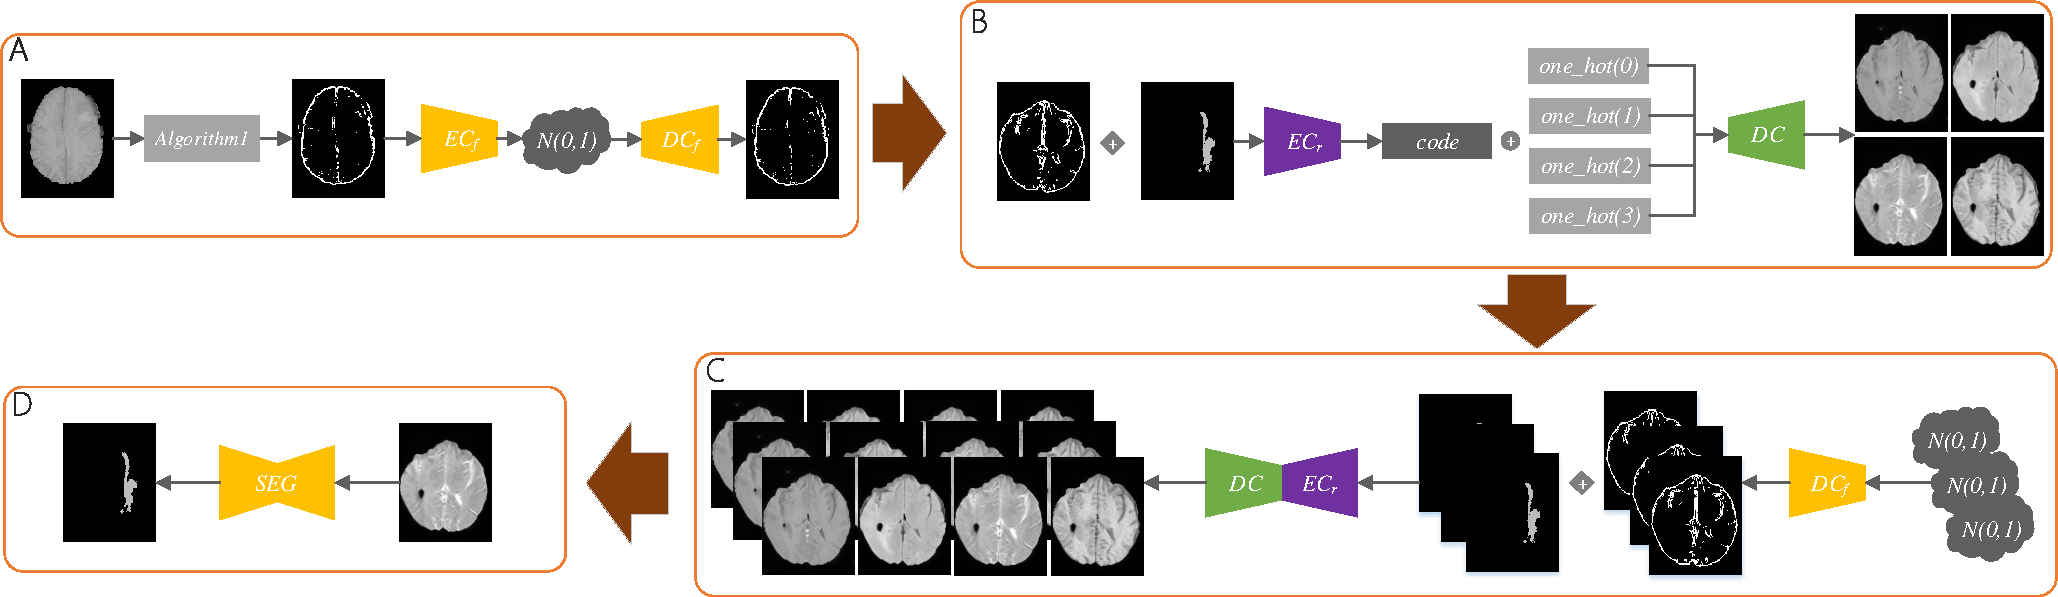
\includegraphics[width=0.95\textwidth]{figures/architecture}
	\caption{The overall architecture. A is the structural feature map extraction and generation stage; B is the multimodal MRI synthesis stage; C is the synthetic datasets construction stage; D is the synthetic data availability verification stage.}
	\label{architecture}
\end{figure*}
As shown in Fig.~\ref{architecture}, our scheme includes four main stages. 
\iffalse
In the structural feature map extraction and generation stage, we will obtain a structural feature map generator that can generate structural feature maps from random normal distribution matrix. 
In the multimodal MRI synthesis stage, we train a conditional generator with input of structural feature maps and lesion labels, which can synthesize MRI of different modalities according to different conditionals.
In the synthetic datasets construction stage, we use the models produced in the previous stages to synthesize registered multimodal MRI from random normal distribution matrixes. 
In the synthetic data availability verification stage, we train and test the lesion segmentors on different datasets constructed from different amounts of synthetic data and real data.
\fi
In the stage A, we will obtain a structural feature map generator that can generate structural feature maps from random normal distribution matrix. 
In the stage B, we train a conditional generator with input of structural feature maps and lesion labels, which can synthesize MRI of different modalities according to different conditionals.
In the stage C, we use the models produced in the previous stages to synthesize registered multimodal MRI from random normal distribution matrixes. 
In the stage D, we train and test the lesion segmentors on different datasets constructed from different amounts of synthetic data and real data.

\subsection{Structural feature map extraction method}
Medical images generated directly from random noise by GAN are difficult to generate realistic structural information. We call the image that provides basic contour and structure information as structural feature map. For example, a retinal vascular distribution map can be regarded as a structural feature map of a retinal image\cite{41costa2017towards}. Structural feature maps can provide necessary basic guidance for the synthesis of medical images. When synthesizing brain MRI, some studies obtain basic structural information from the brain segmentation labels\cite{4shin2018medical}. However, general structural features such as retinal vascular maps and brain segmentation labels require additional data and training before extracting from the original image. 
%To this end, 
To solve this problems, we first design a method for extracting structural feature maps directly from brain MRI, which has the advantages of fast operation, no training, no additional data.

In the traditional digital image processing methods, Roberts operator, Prewitt operator, Sobel operator, etc. are excellent edge detection operators. Sobel operator is often used in processing of brain medical images.
% As shown in Algorithm~\ref{alg:1}, we explore a method to further extract structural feature maps from the edge detection maps generated by Sobel operator.
\begin{algorithm}
	\caption{Structural feature map extraction}
	\label{alg:1}
	\begin{algorithmic}[1]
		\State Input a real image $x$ and pixel threshold $beta$
		\State $f1 = reduce\_min(sobel(x))$
		\State $f2 = reduce\_max(sobel(x))$
		\State $f1 = mean(f1) - f1$
		\State $f2 = f2 - mean(f2)$
		\State $f1 = ones \times (f1 > beta)$
		\State $f2 = ones \times (f2 > beta)$
		\State $f = ones \times ((f1 + f2)> 0.)$
	\end{algorithmic}  
\end{algorithm}
%In Algorithm~\ref{alg:1}
As shown in Algorithm~\ref{alg:1}, we use Sobel operator to extract the horizontal and vertical edge detection maps from a real image. Each edge detection map performs maximum reduce and minimum reduce to obtain two edge detection fusion maps, then each fusion map calculates the difference with average pixel value. The two difference maps are binarized according to the pixel threshold, and the two binary images are summed and then completely binarized. The final result is the structural feature map we need.

\subsection{Structural feature map generation training}
\begin{figure}
	\centering
	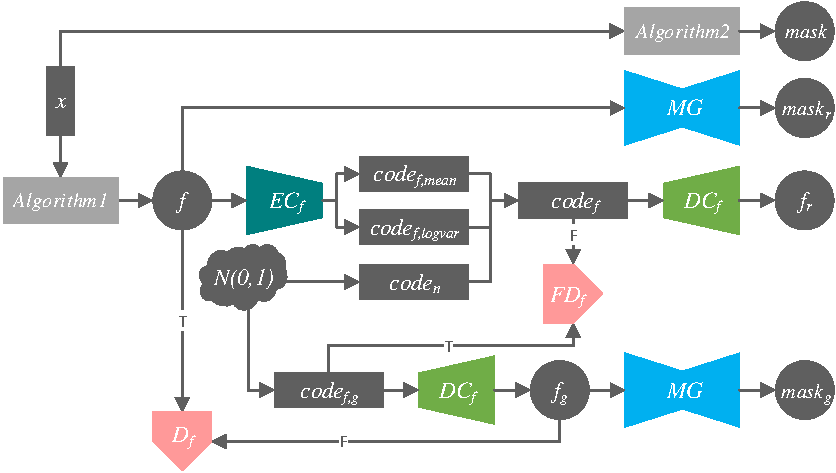
\includegraphics[width=1.0\columnwidth]{figures/feature_train}
	\caption{Structural feature map generation training.}
	\label{feature_train}
\end{figure}
\begin{algorithm}
	\caption{Mask Extraction}
	\label{alg:2}
	\begin{algorithmic}[1]
		\State Input a real image $x$ and the expanded pixel value $p$
		\State $mask = 1.0 - ones \times (x > 0.)$
		\State $new\_size=[x.width() + p, x.length() + p]$
		\State $mask = resize(mask, new\_size)$
		\State $mask = crop\_padding(mask,p)$
	\end{algorithmic}  
\end{algorithm}
When generating the structural feature map, \cite{4shin2018medical} still needs to input real image to get the generated structural feature map, which greatly reduces the diversity of synthetic data. \cite{41costa2017towards} implements a method based on VAE for generating retinal blood vessel distribution maps from multidimensional normal distribution. Drawing on this, we design a hybrid network combining the characteristics of VAE and GAN for generating brain structural feature maps from random normal distribution matrixes, which has better diversity and no additional training data. In addition, we train a generator $MG$ that acquires the brain area masks from the brain structure feature maps for later use to match lesion label. The generator is synchronized with the training of structural feature map generation. During the training of $MG$, the mask extracted by Algorithm~\ref{alg:2} is used as label data. As shown in Fig.~\ref{feature_train}, the specific training processing is as follows:
\begin{itemize}
	\item The structural feature map $f$ is obtained from $x$ using Algorithm~\ref{alg:1}, the mask $mask$ is obtained from $x$ by the Algorithm~\ref{alg:2};
	\item Encode $f$ with VAE encoder $EC_f$ to get $code_{f,mean}$ and $code_{f,logvar}$, then get a random noise $code_n$ from multidimensional normal distribution $\mathcal{N}(0,1^2)$, so the approximate normal distribution matrix  $code_f=code_{f,mean}+exp(0.5\times code_{f,logvar})\times code_n$;
	\item Decode $code_f$ with VAE decoder $DC_f$ to obtain the reconstructed structural feature map $f_r$;
	\item Use mask generator $MG$ to extract mask $mask_r$ from $f$;
	\item Randomly generate a matrix $code_{f,g}$ that obeys normal distribution $\mathcal{N}(0,1^2)$;
	\item Decode $code_{f,g}$ with VAE decoder $DC_f$ to get the generated random structure feature map $f_g$;
	\item Use mask generator $MG$ to extract mask $mask_g$ from $f$;
	\item Structural feature discriminator $D_f$ identifies $f$ and $f_g$ respectively, the former is a positive sample and the latter is a negative sample;
	\item Code matrix distribution discriminator $FD_f$ identifies $code_{f,g}$ and $code_f$, the former is a positive sample and the latter is a negative sample.
\end{itemize}

For the constraint of approximate normal distribution matrix, we do not use the original VAE encoder loss, but add a code matrix distribution discriminator to provide adversarial loss for VAE encoder. Meanwhile, we use $L2$ regular loss to guide the mean matrix with a mean of 0 and the variance deviation matrix with a mean of 1.
The complete loss items are as follows, where $\omega_{i,j}$ is the weight of each loss item, $mean()$ is the mean function: 
\begin{itemize}
	\item{Code matrix distribution discriminator loss} 
	\begin{equation}
		loss_{code,d,f}=\Vert{FD_f(code_{f,g})-1}\Vert_{2}^{2}+\Vert{FD_f(code_f)}\Vert_{2}^{2}
	\end{equation}
	
	\item{Structural feature map discriminator loss} 
	\begin{equation}
		loss_{d,f}=\Vert{D_f(f)-1}\Vert_{2}^{2}+\Vert{D_f(f_g )}\Vert_{2}^{2}
	\end{equation}
	
	\item{Structural feature map adversarial loss} 
	\begin{equation}
		loss_{g,f}=\Vert{FD_f(code_f)-1}\Vert_{2}^{2}+\Vert{D_f(f_g)-1}\Vert_{2}^{2}
	\end{equation}
	
	\item{Code matrix distribution loss } 
	\begin{equation}
	\begin{split}
	loss_{normal}=\Vert{mean(code_{f,mean})}\Vert_{2}^{2}+ \\
	\Vert{mean(exp(0.5\times code_{f,logvar}))-1}\Vert_{2}^{2}
	\end{split}
	\end{equation}
	
	\item{Structural feature map reconstruction loss} 
	\begin{equation}
		loss_{reconstruction,f}=\Vert{f-f_r}\Vert_{2}^{2}+\Vert{f_r\times mask}\Vert_{2}^{2}
	\end{equation}
	
	\item{Mask reconstruction loss}
	\begin{equation}
	\begin{split}
	loss_{reconstruction,mask}=\Vert{mask-mask_r }\Vert_{2}^{2}\\
	+\Vert{f\times mask_r}\Vert_{2}^{2}+\Vert{f_r\times mask_r}\Vert_{2}^{2}+\Vert{f_g\times mask_g}\Vert_{2}^{2}
	\end{split}
	\end{equation}
\end{itemize}
\subsection{Fusion of structural feature map and label}

After generating structural feature map $f_g$, we randomly select appropriate lesion segmentation label $label$, and the lesion segmentation label containing $n$ categories is converted into a one-hot matrix $onehot_l$ of $n$ channels. Each channel corresponds to a segmentation category, the pixel value in each channel is 0 or 1. Each 1 pixel area is registered with each original label segmentation area. At last, we calculate the weighted sum of each channel of $onehot_l$ with $f_g$, and get a new matrix that fuses information of $f_g$ and $label$.

If the structural feature map $f'$ is extracted from random MRI $x$, then the extracted structural features may contain tumor structure information, which may interfere with the tumor information of random label $l$ and affect the syethetic MRI, so $f'$ needs to eliminate the tumor information before fusing with random label $label$, then get the structural feature map $f$ without tumor information, so that the tumor information of syethetic image is only derived from label $label$. We generate a mask without boundary expansion $mask_{l,x}$ for segmentation label $label_x$ of $x$ by Algorithm~\ref{alg:2}, then we have $f=mask_{l,x}\times f'$.

Since the location of randomly selected lesion may appear outside the brain contour of structural feature map, we need to use Algorithm~\ref{alg:2} to obtain the brain region mask $mask$ of structural feature map. If the product of $mask$ and selected $label$ is 0, then the tumor label pixel is inside the brain contour of $mask$, which can be adopted, otherwise the $label$ needs to be re-selected.
\begin{figure*}
	\centering
	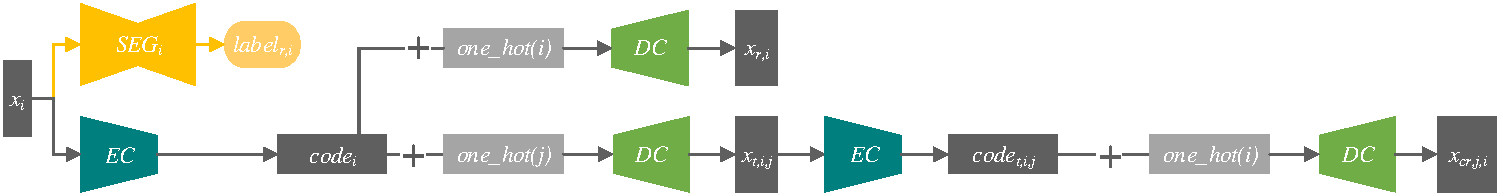
\includegraphics[width=1.95\columnwidth]{figures/trans_train}
	\caption{Reconstruction and translation training.}
	\label{trans_train}
\end{figure*}
\iffalse
\subsection{Reconstruction and translation training}
We perform reconstruction and translation training on real data and synchronize with multimodal MRI synthesis training in subsequent sections. These trianings constrain each component to complete our specified tasks in multimodal MRI synthesis process. In addition, we also use a code matrix distribution discriminator $FD$ to guide the consistency of code matrixes distribution between the two training processes. All discriminator components are updated independently, the discriminator training process is shown in Fig.~\ref{train_D}.

\begin{figure*}
	\centering
	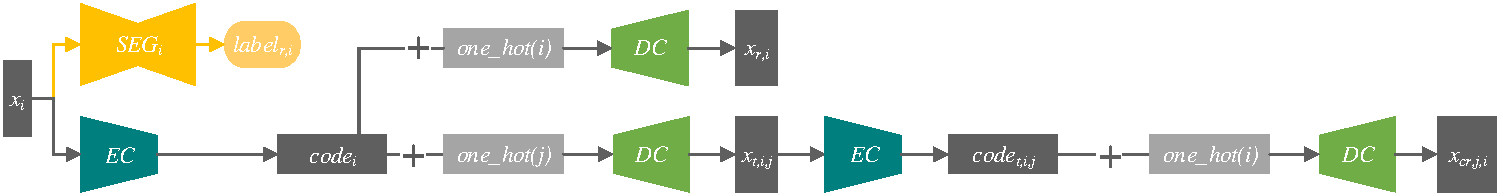
\includegraphics[width=1.75\columnwidth]{figures/trans_train}
	\caption{Reconstruction and translation training.}
	\label{trans_train}
\end{figure*}

As shown in Fig.~\ref{trans_train}, when the MRI is reconstructed and translated, encoder $EC$ encodes real MRI $x_i$ of modality $i$ to obtain semantic feature map $code_{i}$, then it is concatenated to different conditional matrixes and obtain all the modalities through decoder $DC$. In cycle-reconstruction, we use encoder to re-encode all the obtained translation images, concatenate all re-encoded semantic feature maps with conditional vector of modality $i$, and finally decode them by decoder to get cycle-reconstruction image $x_{rc,j,i}$. In the above process, we use the lesion label $l_i$ of original input modality $x_i$ as the supervised label for lesion generation training, and use lesion label generation components for $x_i$ to get $l_{r,i}$.

The detailed losses are as follows, where $x_{t,j,i}$ refers to MRI $x_i$ of modality $i$ translated by modality $j$; $d_{t, j, i}$ and $c_{t, j, i}$ are the True/False discrimination and category discrimination results of discriminator $D$ for $x_{t, i, j}$; $code_{t,i,j}$ represents semantic feature map obtained from $x_{t,i,j}$ by encoder:
\begin{itemize}
	\item{Discriminator loss}
	\begin{equation}
	\begin{split}
	loss_{d,1}=&\sum\limits_{j=0}\sum\limits_{i=0, i\neq j}(\Vert{d_{t,j,i}}\Vert_{2}^{2}+\Vert{c_{t,j,i}-i}\Vert_{2}^{2})\\
	&+\sum\limits_{i=0}(\Vert{FD(code_{i})-1}\Vert_{2}^{2})
	\end{split}
	\end{equation}
	
	\item{Adversarial and category guidance loss}
	\begin{equation}
	loss_{g,1}=\sum\limits_{j=0}\sum\limits_{i=0, i\neq j}(\Vert{d_{t,j,i}-1}\Vert_{2}^{2}+\Vert{c_{t,j,i}-i}\Vert_{2}^{2})
	\end{equation}
	
	\item{MRI reconstruction loss}
	\begin{equation}
	loss_{reconstruction}=\sum\limits_{i=0}(\Vert{x_i-x_{r,i}}\Vert_{2}^{2})
	\end{equation}
	
	\item{MRI cycle-reconstruction loss}
	\begin{equation}
	\begin{split}
	loss_{cycle}=\sum\limits_{j=0}\sum\limits_{i=0, i\neq j}(\Vert{x_i-x_{cr,j,i}}\Vert_{2}^{2})+\\
	\sum\limits_{k=0}\sum\limits_{j=0,j\neq k}\sum\limits_{i=0, i\neq j,i\neq k}(\Vert{x_{cr,j,i}-x_{cr,k,i}}\Vert_{2}^{2})
	\end{split}
	\end{equation}
	
	\item{Semantic consistency loss}
	\begin{equation}
	loss_{code,1}=\sum\limits_{j=0}\sum\limits_{i=0, i\neq j}(\Vert{code_i-code_{t,i,j}}\Vert_{2}^{2})
	\end{equation}
	
	\item{Lesion segmentation loss}
	\begin{equation}
	loss_{lesion,1}=\sum\limits_{i=0}\Vert{label_i-label_{r,i}}\Vert_{2}^{2}
	\end{equation}
\end{itemize}
\fi

\subsection{Multimodal MRI synthesis training}
\begin{figure*}
	\centering
	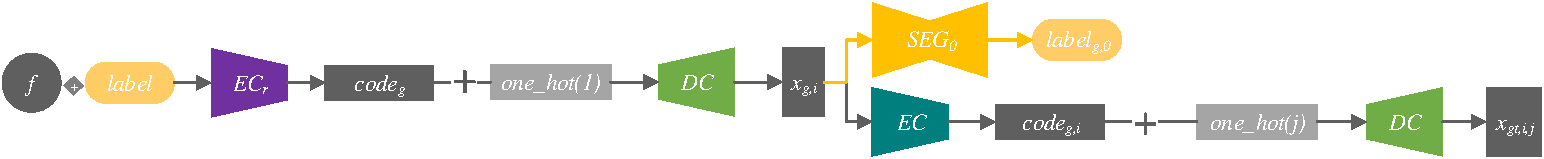
\includegraphics[width=1.98\columnwidth]{figures/mm_mri_generate}
	\caption{Synthesis of multimodal MRI.}
	\label{mm_mri_generate}
\end{figure*}

\begin{figure}
	\centering
	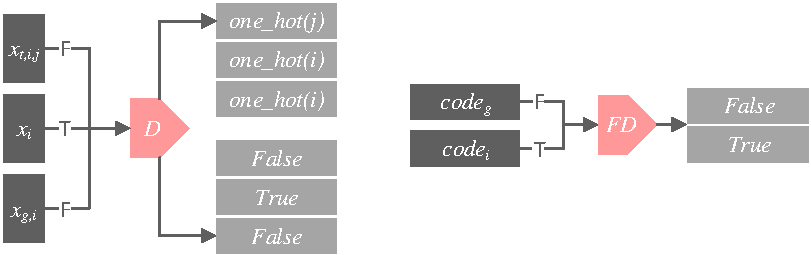
\includegraphics[width=0.95\columnwidth]{figures/D}
	\caption{Discriminator training during reconstruction and translation training on real MRI and multimodal MRI generation training.}
	\label{train_D}
\end{figure}
Before the multimodal MRI synthesis process, We perform reconstruction and translation training on real data. These trianings constrain each component to complete our specified tasks in multimodal MRI synthesis process. 
As shown in Fig.~\ref{trans_train}, when the MRI is reconstructed and translated, encoder $EC$ encodes real MRI $x_i$ of modality $i$ to obtain semantic feature map $code_{i}$, then it is concatenated to different conditional matrixes and obtain all the modalities through decoder $DC$. In cycle-reconstruction, we use encoder to re-encode all the obtained translation images, concatenate all re-encoded semantic feature maps with conditional vector of modality $i$, and finally decode them by decoder to get cycle-reconstruction image $x_{rc,j,i}$. In the above process, we use the lesion label $l_i$ of original input modality $x_i$ as the supervised label for lesion generation training, and use lesion label generation components for $x_i$ to get $l_{r,i}$. 

What's more, we also use a code matrix distribution discriminator $FD$ to guide the consistency of code matrixes distribution between the two training processes. All discriminator components are updated independently, the discriminator training process is shown in Fig.~\ref{train_D}.

In addition to the loss settings in CycleGAN, we also design the following losses for reconstruction and translation training:
\begin{itemize}
	\item{Feature Discriminator loss}
	\begin{equation}
	\begin{split}
	loss_{fd}=\sum\limits_{i=0}(\Vert{FD(code_{i})-1}\Vert_{2}^{2})
	\end{split}
	\end{equation}
	\item{Lesion segmentation loss}
	\begin{equation}
	loss_{lesion,1}=\sum\limits_{i=0}\Vert{label_i-label_{r,i}}\Vert_{2}^{2}
	\end{equation}
\end{itemize}

The multimodal MRI synthesis process is shown in Fig.~\ref{mm_mri_generate}. First, we extract the structural feature map $f$ from real MRI by Algorithm~\ref{alg:1}, and randomly select the real lesion label $label$ for fusion. The fusion map contains basic anatomical information and lesion information of the target site. 
We use a fusion map encoder $EC_r$ to encode fusion map and obtain the semantic feature map. The semantic feature map is concatenated to different one-hot conditional matrixes as input to MRI decoder, then obtains synthetic image of different modalities. These synthetic images are then performing modal translation process between each other by MRI encoder and MRI decoder. We use adversarial loss and category guidance loss provided by MRI discriminator to constrain synthetic image to approximate real MRI, and constrain the consistency of all semantic feature maps and translation images by loss, thus ensuring the mutual registration of synthetic multimodal MRI. In addition, we use the lesion label generation components to segment the tumor lesion segmentation labels from each synthetic MRI to ensure that the synthetic multimodal images have synthesized corresponding lesion content based on the input lesion label. The lesion label generation components are only trained by real data in reconstruction and translation training. 

The specific loss items of the multimodal MRI synthesis process are as follows, where $d_{i}$ and $c_{i}$ are the True/False discrimination and category discrimination of the discriminator $D(x_i)$, $d_{g, i}$,$c_{g,i}$ is the output of $D(x_{g,i})$. $x_{g,i}$ is the synthetic image of modality $i$, $x_{gt,j,i}$ is the synthetic image of the modality $i$ translated by synthetic image of modality $j$. $code_g$ is the semantic feature map obtained by fusion map encoder$EC_R$, $code_{g,i}$ is the semantic feature map encoded from $x_i$. $l$ is the input label, $l_{g,i}$ is the label obtained by lesion label generation component from $x_{g,i}$. $f$ is the input structural feature map, $f_{g,i}$ is the structural feature map extracted from $x_{g,i}$ by Algorithm~\ref{alg:1}:
\begin{itemize}
	\item{Discriminator loss }
	\begin{equation}
	\begin{split}
		loss_{d}=&\sum\limits_{i=0}(\Vert{d_{i}-1}\Vert_{2}^{2}+\Vert{d_{g,i}}\Vert_{2}^{2}+\Vert{c_{i}-i}\Vert_{2}^{2}+\\
		&\Vert{c_{g,i}-i}\Vert_{2}^{2})+\Vert{FD(code_{g})}\Vert_{2}^{2}
	\end{split}
	\end{equation}
	
	\item{Adversarial and category guidance loss}
	\begin{equation}
		loss_{g}=\sum\limits_{i=0}(\Vert{d_{g,i}-1}\Vert_{2}^{2}+\Vert{c_{g,i}-i}\Vert_{2}^{2})+\Vert{FD(code_{g})-1}\Vert_{2}^{2}
	\end{equation}
	
	\item{Structural feature map consistency loss}
	\begin{equation}
		loss_{f}=\sum\limits_{i=0}(\Vert{f-f_{g,i}}\Vert_{2}^{2})
	\end{equation}
	
	\item{Lesion generation loss}
	\begin{equation}
		loss_{lesion,2}=\sum\limits_{i=0}(\Vert{label-label_{g,i}}\Vert_{2}^{2})
	\end{equation}
	
	\item{MRI registration loss}
	\begin{equation}
		loss_{registration}=\sum\limits_{j=0}\sum\limits_{i=0,i\neq j}(\Vert{x_{g,i}-x_{gt,j,i}}\Vert_{2}^{2})
	\end{equation}
	
	\item{Semantic consistency loss}
	\begin{equation}
	\begin{split}
		loss_{code}=&\sum\limits_{i=0}(\Vert{code_g-code_{g,i}}\Vert_{2}^{2})+\\
		&\sum\limits_{j=0}\sum\limits_{i=0, ,i\neq j}(\Vert{code_{g,i}-code_{g,j}}\Vert_{2}^{2})
	\end{split}
	\end{equation}
	
\end{itemize}

\subsection{Lesion generation guidance method}
\label{label gen methods}
As shown in Fig.~\ref{segmentation}, we design the following three lesion label generation components to provide guidance loss for lesion generation in multimodal MRI synthesis training:
\begin{enumerate}
	\item{Single segmentor} 
	
	Each MRI modality  is segmented by a common complete segmentor $SEG$.
	\item{Single lesion encoder + multiple lesion decoders} 
	
	Each MRI modality  is segmented by a segmentor which is combined by a common lesion encoder $EC_{l}$ and different lesion decoders $EC_{l,i}$. 
	\item{Multiple segmentors} 
	
	Each MRI modality  is segmented by a different complete segmentor $SEG_i$.
\end{enumerate}
The loss item of the above three methods in reconstruction and translation training is consistent with the loss item described above. And in the generation training, it only provides the same lesion label generation loss for MRI synthesis components, no learning.

\begin{figure}
	\centering
	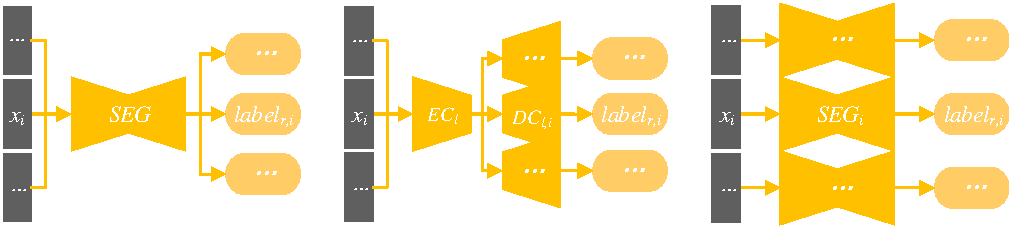
\includegraphics[width=0.98\columnwidth]{figures/segmentation}
	\caption{Lesion segmentation.}
	\label{segmentation}
\end{figure}
Besides, we also train the segmentors of these three methods independently. In different experiments, we will train the segmentor in each method with different amounts of synthetic data or real data. The loss function of the training is as follows, where $label_i$ is the supervised label and $label_{r,i}$ is the segmentation result:
\begin{equation}
	loss_{segmentation}=\sum\limits_{i=0}\Vert{label_i-label_{r,i}}\Vert_{2}^{2}
\end{equation}

\subsection{Construction of synthetic datasets}
\label{make dataset}
\begin{figure*}
	\centering
	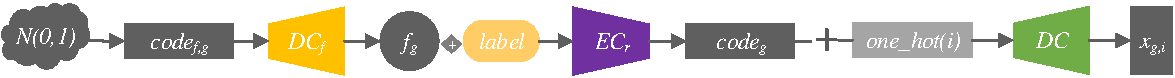
\includegraphics[width=1.98\columnwidth]{figures/make_data}
	\caption{Construction of synthetic datasets.}
	\label{make_data}
\end{figure*}
As shown in Fig.~\ref{make_data}, we can generate any number of structural feature maps from random normal distribution matrix through the trained structural feature map decoder. Then, we randomly scaled, rotated, translated, flipped the original label set to get a random lesion label set. We then fuse the generated structural feature map with randomly selected label from the random lesion label set. Like training stage, we can select suitable labels by obtaining masks from structural feature maps through the mask generator $MG$.

Due to the influence of the operation that removing tumor information in training, there are some structural feature maps with poor quality that brain contour is not closed, so we design a structural feature map filtering algorithm for this. First, we use the generator $MG$ to generate the mask of structural feature map. Then, we perform Gaussian blur\cite{92wink2004denoising} on the structural feature map, and use the contour search algorithm and filling algorithm provided by OpenCV\footnote{https://opencv.org/} to obtain all the closed contours of the Gaussian blur image and fill them. So we get another mask by the traditional algorithm. Finally, we calculate the Mean Absolute Error (MAE) of the two masks. If the MAE is lower than the threshold we set, that means the main brain contour of the structural feature map is relatively complete, and the feature map can be used; otherwise, it means that the mask obtained by traditional algorithm is hollow inside and quite different with the mask generated by generator, so it needs to be regenerated. The algorithm is expressed as Algorithm~\ref{alg:3}.
\begin{algorithm}
	\caption{Structural Feature Map Filtering}
	\label{alg:3}
	\begin{algorithmic}[1]
		\State Input a MAE threshold $mae$
		\State \textbf{function} $get\_mask(f)$
		\State \indent$contours = OpenCV.findContours(f)$
		\State \indent$mask =OpenCV.drawContours(f,contours)$
		\State \indent\textbf{return} $mask$
		\State \textbf{do} 
		\State \indent$f = DC_f()$
		\State \indent$m = MG(f)$
		\State \indent$m'= get\_mask(f)$
		\State \textbf{while} $MAE(m',m) <= mae$
	\end{algorithmic}  
\end{algorithm}

In the systhetic multimodal MRI dataset, there are still samples with poor quality of lesion generation. At this point, we segment our synthetic MRI data through the lesion segmentor pre-trained on real data. We filter according to the segmentation evaluation score(default threshold is 0.95 on Dice Score). After multiple filtering, we obtain the final synthetic dataset consisting of structural feature maps, masks, lesion segmentation labels, and multimodal MRI.

\section{EXPERIMENTS}
\subsection{BRATS2015 dataset}
We use the open dataset BRATS2015\cite{91menze:hal-00935640} for experiments, which has four registered modalities of T1/T2/T1c/Flair. The training dataset contains 274 3D MRIs per modality, with the size of 155$\times$240$\times$240, and 274 tumor segmentation labels of the same size. We divide the sample into a training set and a test set by 9:1, and construct a 2D data set from 50 slices of each 55-105 of the 3D MRI. In data preprocessing, we have standardized each image.

\subsection{BRATS synthetic dataset}
We construct a registered synthetic dataset with tumor labels containing four modalities of T1/T2/T1c/Flair using the method in Section~\ref{make dataset}. The size of the synthetic dataset samples are consistent with the BRATS2015 dataset, but the number of samples can be any number according to the needs of the experiment.

\subsection{BRATS enhanced dataset}
We perform random scaling, rotation, translation, flipping, etc. on the original BRATS2015 dataset to obtain enhanced data. The size of the enhanced dataset sample is consistent with the BRATS2015 dataset, but the number of samples can be any number according to the needs of the experiment.

\subsection{Training settings}
The iteration number of each experiment is equal to 100 epochs of the BRATS2015 training dataset. The learning rate is 1e-4 without weight decay. We use Adam optimizer with beta1 of 0.5 and perform a Dropout of 0.1 on the input layer, batch size is 1. We use Dice Score \cite{95dice1945measures} and Mean Square Error (MSE)\cite{94prasad1990the} to evaluate the segmentation results. The evaluation results are the average of the 4 modal results on the 2D images, and each experiment is trained four times to retain the best results.

\subsection{Experiments of lesion generation methods}
\label{label gen methods tests}
As shown in Table~\ref{label_test}, we train 4 tumor lesion segmentors using the multiple segmentors method on BRATS2015 training dataset and test them on BRATS2015 test dataset. Then we use the trained segmentors to segment the unfiltered synthetic data from different lesion generation guidance methods.
\begin{table}
	\begin{center}
		{\caption{Lesion generation methods experiments.}\label{label_test}}
		\begin{tabular}{lcccc}
			\hline
			\rule{0pt}{12pt}
			segmentation schemes&testing dataset &MSE   &Dice Score
			\\
			\hline
			\\[-6pt]
			\quad 4 $SEG$&real 		   				&0.026 &0.915 \\					
			\quad 1 $SEG$&synthetic     			&0.053 &0.741 \\			
			\quad 1 $EC_{l}$ + 4 $DC_{l}$&synthetic     	&0.055 &0.808 \\		
			\quad 4 $SEG$&synthetic     			&\textbf{0.043} &\textbf{0.838} \\
			\hline
			\\[-6pt]
		\end{tabular}
	\end{center}
\end{table}
\subsection{Experiments of synthetic data availability}
As shown in Table~\ref{availability_test}, we mix real BRATS2015 training data with BRATS synthetic data in different amounts, then use the mixed dataset for segmentation training using the multiple segmentors method, and evaluate the segmentation ability of the model on real BRATS2015 test dataset. All experiments have been fully trained with the same number of iterations, which equal to the number of 100 epochs on BRATS2015 training dataset. At the same time, we set up three data mixing modes: random mixing, real data training first, and synthetic data training first.In real first experiments and synthetic first experiments, the training iteration number of data from different sources is proportional to the amount of data. Except the conditions in tabel, other conditions are identical.
\section{RESULTS}
\iffalse
\begin{figure}
	\centering
	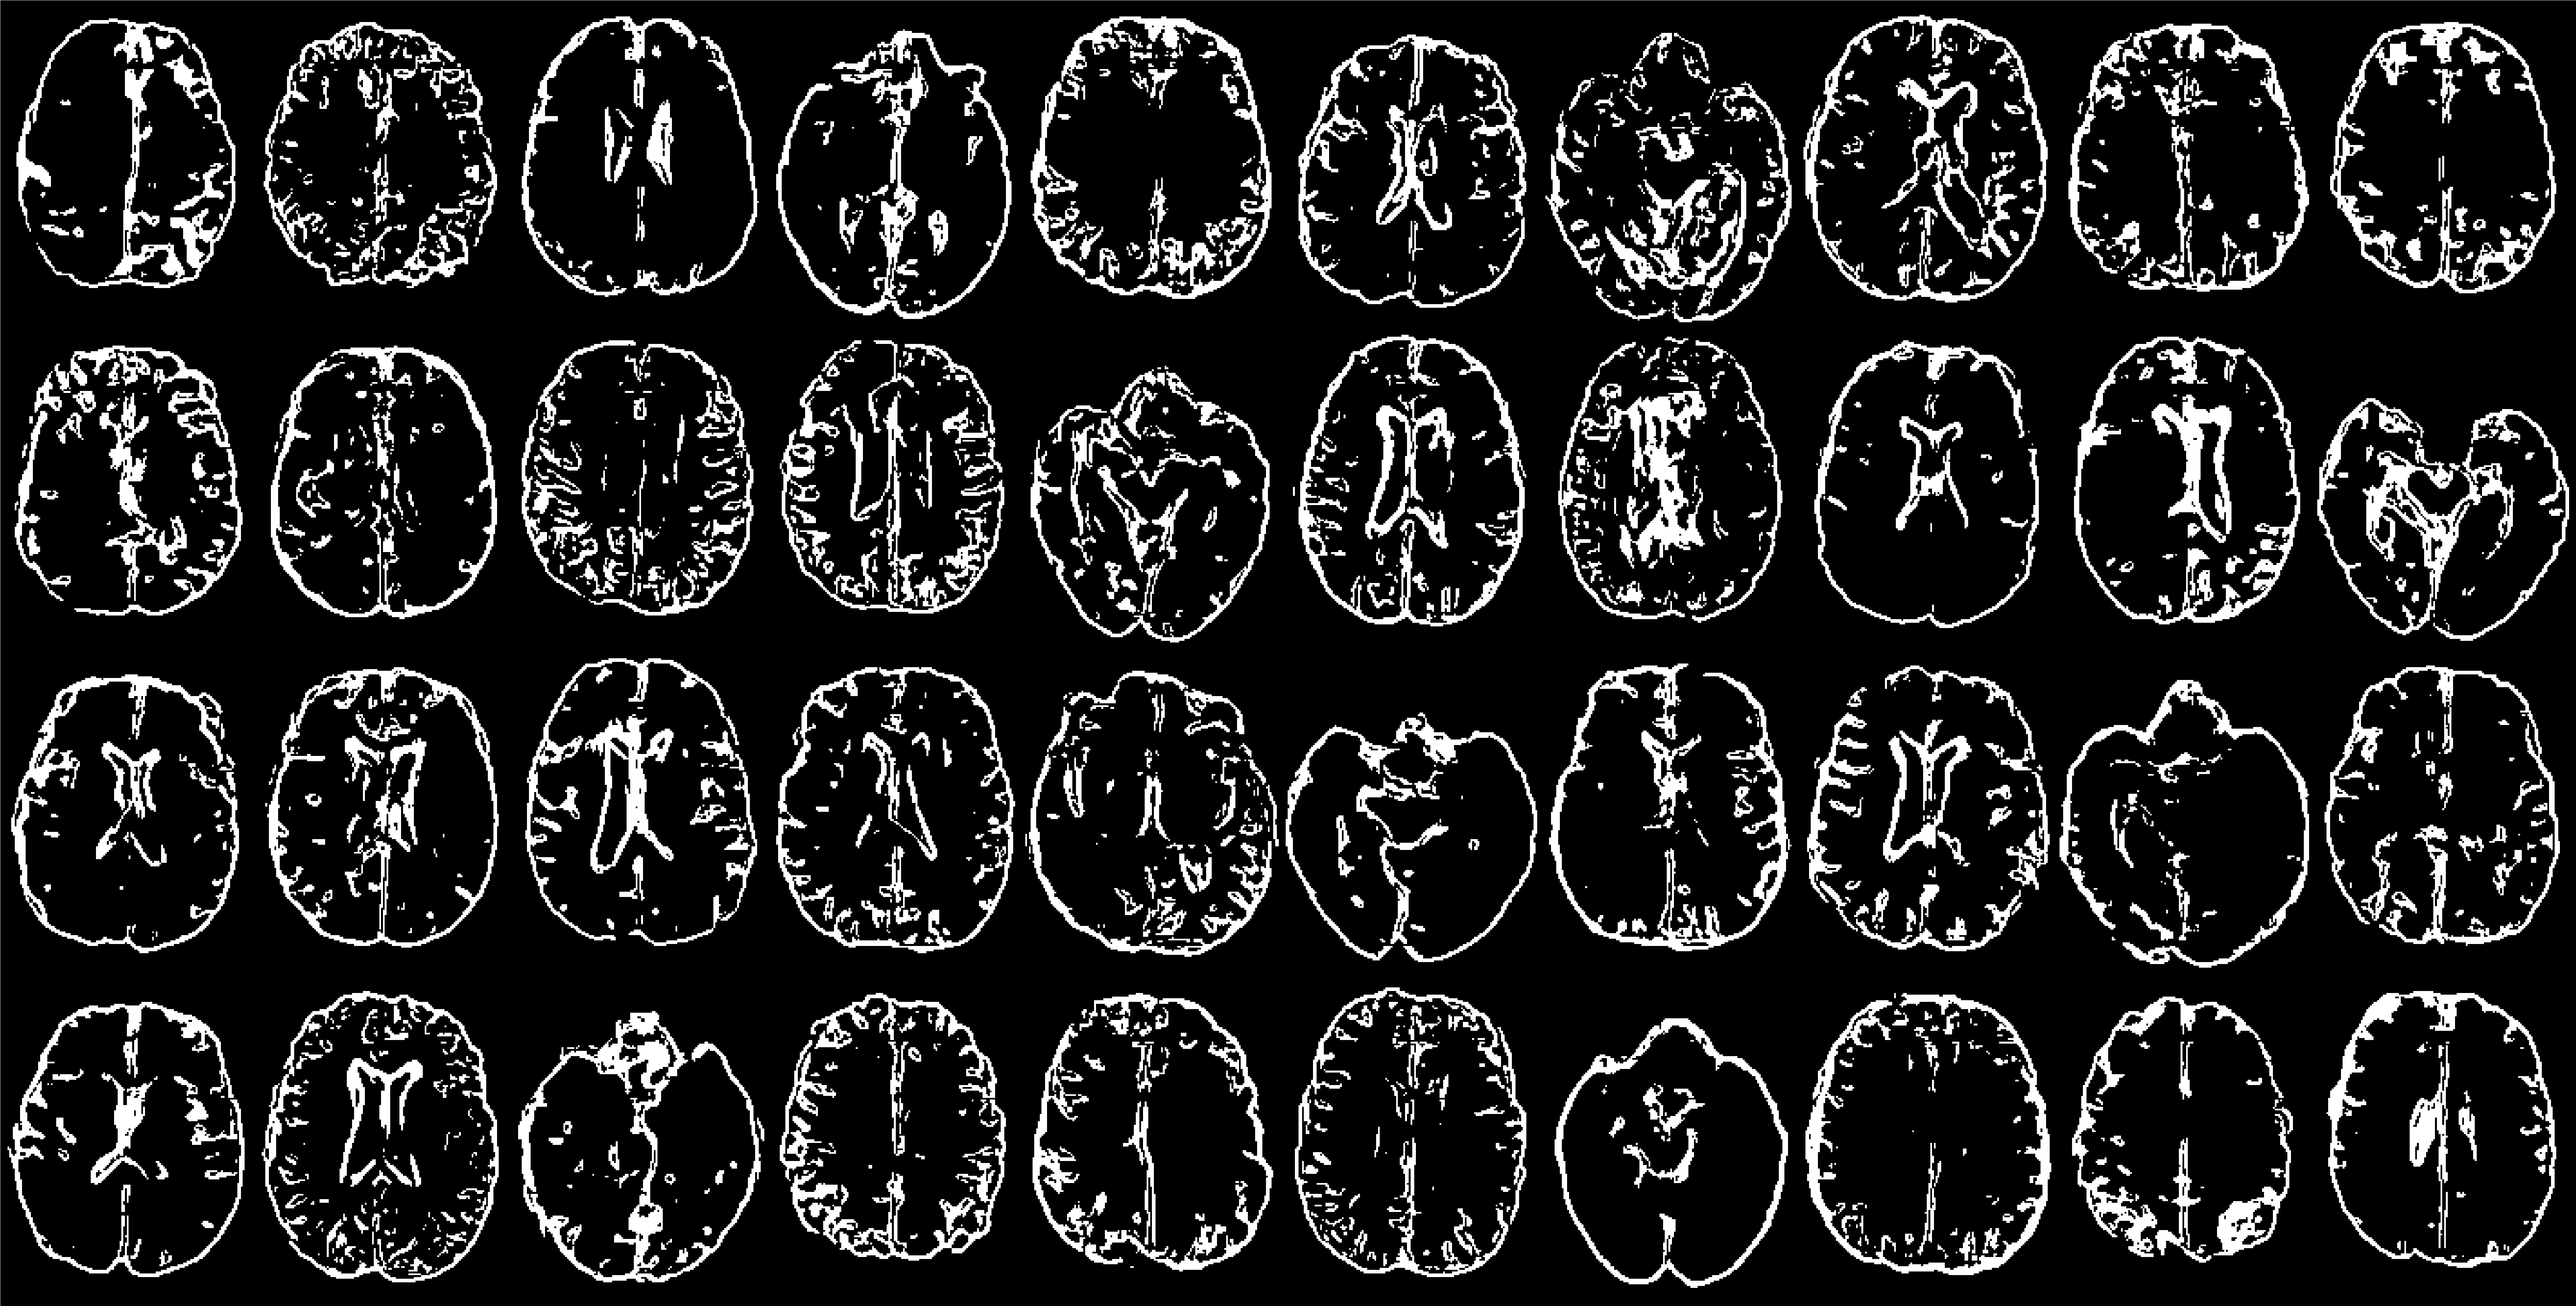
\includegraphics[width=0.95\linewidth]{figures/Fs}
	\caption{Synthetic structural feature maps.}
	\label{generated_f}
\end{figure}
\fi
%Fig.~\ref{generated_f} shows the examples of the structural feature map generated from random normal distribution matrix. 
Fig.~\ref{generated_mri} shows the examples of images obtained from all stages.
\begin{figure}
	\centering
	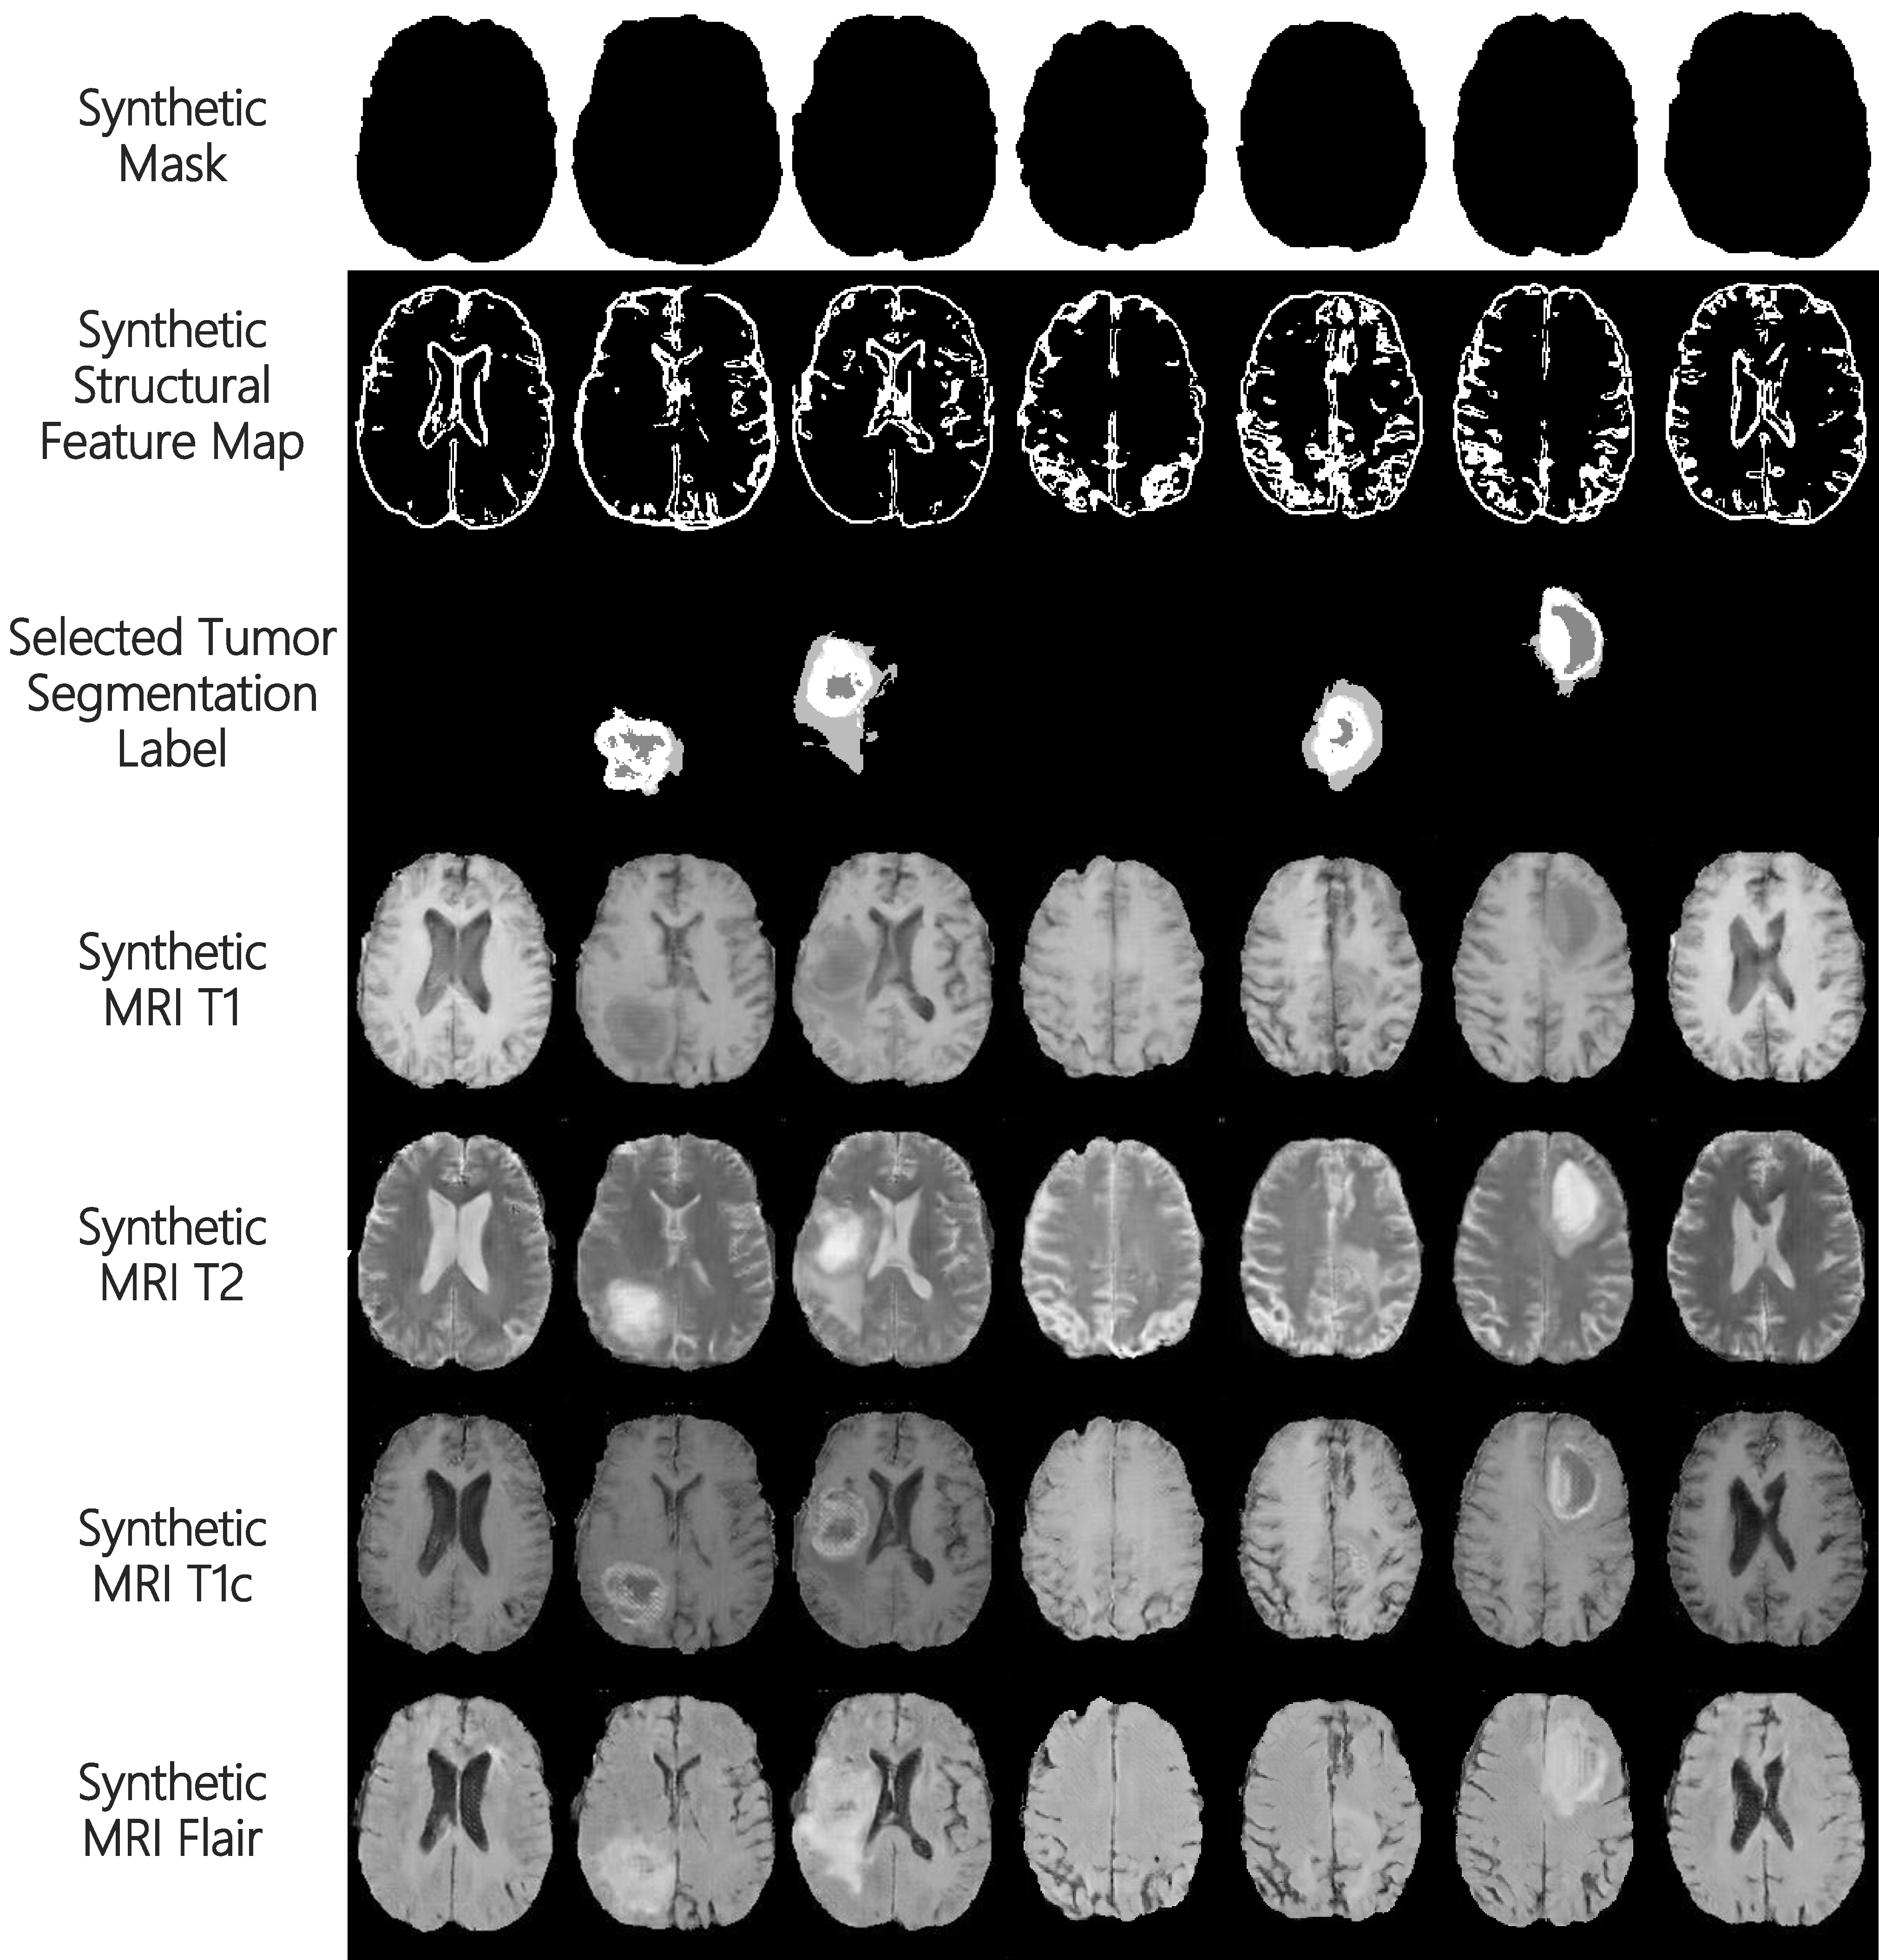
\includegraphics[width=0.98\linewidth]{figures/F_to_MRI}
	\caption{Multimodal MRIs systhesized from structural feature maps and lesion labels.}
	\label{generated_mri}
\end{figure}
\subsection{Results of lesion generation methods}
\begin{table*}[t]
	\begin{center}
		{\caption{Synthetic data availability verification experiments.}\label{availability_test}}
		\begin{tabular}{lllllcc}
			\hline
			\rule{0pt}{12pt}
			NO. &real data &synthetic data & enhanced data  & mixing modes  & MSE &Dice Score\\
			\hline
			\\[-6pt]
			\quad 1 & $\times$1  	 	& 0 		&0 			&- &0.026 &0.915 \\
			\quad2 & $\times$50\% 	 & 0  		&0 			&- &0.032 &0.902 \\
			\quad3 &0 	 	 & $\times$1  	&0 			&- &0.205 &0.708 \\
			\quad4 &0 	 	 & $\times$2  	&0 			&random mixing &0.206 &0.736 \\
			\quad5 &0 		 & $\times$3  	&0 			&random mixing &0.205 &0.754 \\
			\quad6 & $\times$10\% 	 & $\times$1  	&0 			&synthetic first &0.031 &0.908 \\
			\quad7 & $\times$10\% 	 & $\times$2   &0 			&synthetic first &0.028 &0.907 \\
			\quad8 & $\times$10\% 	 & $\times$3   &0 			&synthetic first &0.030 &0.907 \\	
			\quad9 & $\times$20\% 	 & $\times$80\% 	&0  		&random mixing &0.041 &0.850 \\
			\quad10& $\times$50\% 	 & $\times$50\% 	&0  		&random mixing &0.031 &0.904 \\
			\quad11& $\times$80\% 	 & $\times$20\% 	&0  		&random mixing &0.024 &0.935 \\
			\quad12& $\times$1 	 	& $\times$20\% &0  		&random mixing &0.025 &0.921 \\
			\quad13& $\times$1 	 	& $\times$50\% &0  		&random mixing &\textbf{0.023} &\textbf{0.939} \\
			\quad14& $\times$1 	 	& $\times$80\% &0  		&random mixing &0.026 &0.916 \\
			\quad15& $\times$1 	 	& $\times$1    &0   		&random mixing &0.027 &0.913 \\
			\quad16& $\times$1 	 	& $\times$2   &0 			&random mixing &0.033 &0.901 \\
			\quad17& $\times$1 	 	& $\times$3   &0 			&random mixing &0.034 &0.897 \\	
			\quad18& $\times$1 	 	&0 		&  $\times$20\%	 	&random mixing &0.027 &0.911 \\
			\quad19& $\times$1 	 	&0 		&  $\times$50\% 	&random mixing &0.025 &0.927 \\
			\quad20& $\times$1    	&0 		&  $\times$80\% 	&random mixing &0.026 &0.920 \\
			\quad21& $\times$1 	 	&0 		&  $\times$1    &random mixing &0.026 &0.915 \\
			\quad22& $\times$1 	 	&0 		&  $\times$2   &random mixing &0.032 &0.898 \\
			\quad23& $\times$1 	 	&0 		&  $\times$3   &random mixing &0.036 &0.885 \\			
			\quad24& $\times$1 	 	& $\times$1 	&0  		&real first &0.195 &0.795 \\
			\quad25& $\times$1 	 	& $\times$1 	&0  		&synthetic first &\textbf{0.021} &\textbf{0.940}
			\\
			\hline
			\\[-6pt]
		\end{tabular}
	\end{center}
\end{table*}
As shown in Table~\ref{label_test}, segmentation test results of the segmentor trained on real data have reached MSE of 0.026 and Dice Score of 0.915. From results, three different lesion label generation methods have achieved good segmentation results, where the multiple segmentors method is the best. 

\subsection{Results of Synthetic Data Availability}
As shown in Table~\ref{availability_test}, the results of experiment NO.3-NO.5 show that the synthetic data can not completely replace real data in training.           
The results of NO.6-NO.8 show that the performances of pre-training with a large amount of synthetic data and fine-tuning on a small amount of real data are similar to those of training with complete real data.  
In NO.9-NO.11, the results of different mixing ratios are also quite different. When the two ratios are close, the segmentation results are similar to NO.1. When the proportion of synthetic data is high, the synthetic data will interfere with the learning of real data, and the result is lower than that of NO.1. When the proportion of synthetic data is low, the generalization ability of the model can be improved by synthetic data, and the result is higher than NO.1.           
In NO.12-NO.17, we further try to add synthetic data of different quantities to real data, which show that adding a small amount of synthetic data can enhance the learning, and the more synthetic data, the better the enhancement effect, but when the synthetic data reaches a certain percentage and then continue to increase, it achieves the opposite effect. 
In NO.18-NO.23, we compare the enhancement effect of synthetic data and enhanced data generated by usual data enhancement methods. We found that the two are similar but not equal in the trend between  enhancement effect and the increase in data amount.Overall, the enhanced data is more robust in terms of the sensitivity of model to the amount of enhanced data, but the enhancement effect upper limit of synthetic data is much higher than that of enhanced data.  
We compared NO.24-NO.25 with NO.15 and found that the performance of synthetic data is the best when it is used as pre-training data, and the performance is poor when it is used as supplementary training data. when using as enhanced data to mixed with real data, the synthetic data can also achieve certain enhancements.

Generally, if there are a large amount of real data, a small amount of synthetic data can be used as enhanced data, or a large amount of synthetic data can be used for pre-training and then training on real data. And if there are less real data, a large number of synthetic data can be used for pre-training, then fine-tuned on a small amount of real data, whose results can compete with the results on complete real data, and this conclusion is consistent with \cite{4shin2018medical}. We do not recommend using synthetic data completely for training, and also do not recommend using synthetic data for supplementary training.


\section{CONCLUSION}
In short, We propose a structural feature map extraction method to extract anatomical structure information directly from medical images without training or additional label data;
We propose a structure feature map generation method to generate structural feature maps from multidimensional normal distribution matrixes;
we realize the synthesis of registered multimodal MRI from random normal distribution matrix through unsupervised training, which can add the lesion information freely;
We verify that synthetic MRI can be used as pre-training data or enhanced data for intelligent medical image processing tasks and can significantly improve the generalization ability of the model through lesion segmentation experiments.
\iffalse
In this paper, our contributions are as follows:
\begin{itemize}
	\item We propose a structural feature map extraction method to extract anatomical structure information directly from medical images without training or additional label data;
	\item We propose a structure feature map generation method to generate structural feature maps from multidimensional normal distribution matrixes;
	\item We realize the synthesis of registered multimodal MRI with corresponding lesion information from structural feature map and randomly selected lesion labels;
	\item We verify that synthetic data can be used as pre-training data or enhanced data for intelligent medical image processing tasks through a number of data availability tests.
\end{itemize}
\fi
\ack We would like to thank the 

\bibliography{refer}
\end{document}
%%%%%%%%%%%%%%%%%%%%%%%%%%%%%%%%%%%%%%%%%%%%%%%%%%%%%%%%%%%%%%%%%%%%%%
